\documentclass[aspectratio=169]{beamer}
\usepackage{will_handley}

\usepackage{tikz}
\newcommand{\av}[2][]{\left\langle #2\right\rangle_{#1}}
\newcommand{\PR}{\mathcal{P}_\mathcal{R}}
\newcommand{\Pknotj}[1]{\mathcal{P}_{#1}}
\newcommand{\Nknots}{N_\text{knots}}
\newcommand{\nlive}{n_\text{live}}

\newcommand{\movablecross}[1]{%
  \draw[->](#1) -- ++(0:\croslen);
  \draw[->](#1) -- ++(90:\croslen);
  \draw[->](#1) -- ++(180:\croslen);
  \draw[->](#1) -- ++(270:\croslen);
  \fill[red!70!black] (#1) circle (2pt);
}

\newcommand{\movablevert}[1]{%
  \draw[->](#1) -- ++(90:\croslen);
  \draw[->](#1) -- ++(270:\croslen);
  \fill[red!70!black] (#1) circle (2pt);
}

% Commands
% --------
% - \arxiv{arxiv number}
% - \cols{width}{lh column}{rh column}
% -  \begin{fig(left|right)}[fractional width (e.g 0.6) ]{name of image}
%        content of other column
%    \end{fig(left|right)}

% Talk details
% ------------
\title{Statistical methods in cosmology}
%\subtitle{<+subtitle+>}
\date{12\textsuperscript{th} April 2022}

\begin{document}

\begin{frame}
    \titlepage
\end{frame}

\begin{frame}
    \frametitle{Lessons from the CMB}
    \begin{columns}
        \column{0.5\textwidth}
        \begin{itemize}
            \item 21cm global signal detection is superficially similar to detecting the primordial CMB.
            \item Both are attempted to detect tiny $\sim 10^{-5}$ cosmological signals hidden beneath a large ``uninteresting'' foreground.
            \item Both measurements are frustrated by complicated contaminants.
            \item Both are amenable to a Bayesian analysis.
        \end{itemize}
        \column{0.5\textwidth}
        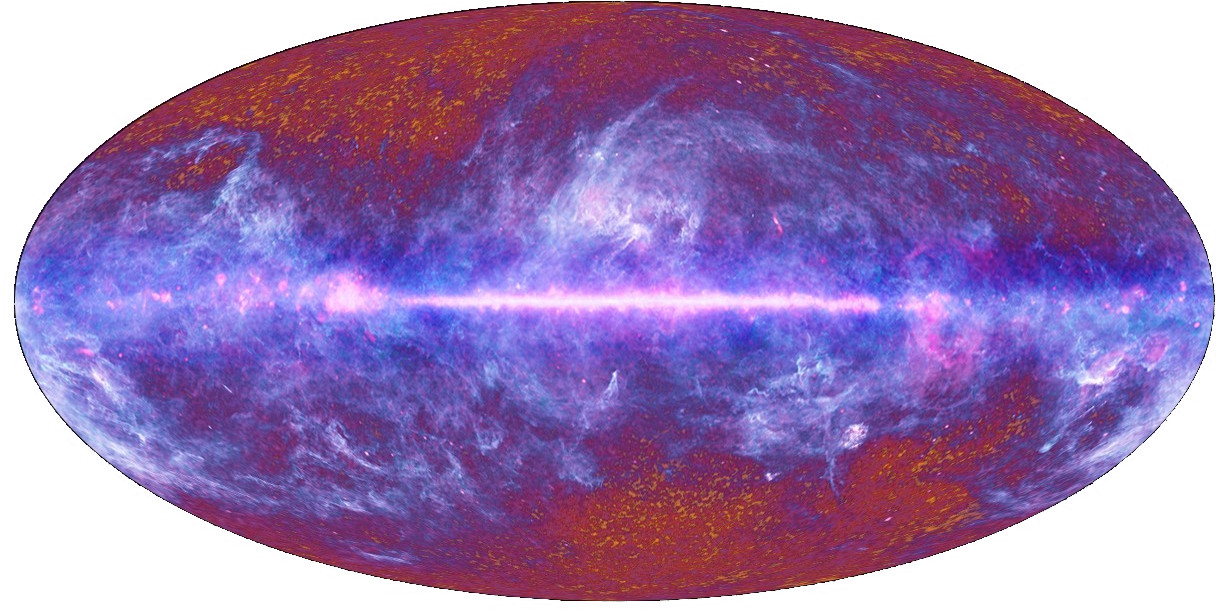
\includegraphics[width=\textwidth]{figures/9HXKAsNw5LtSRHFPWfeqiB.jpg}
        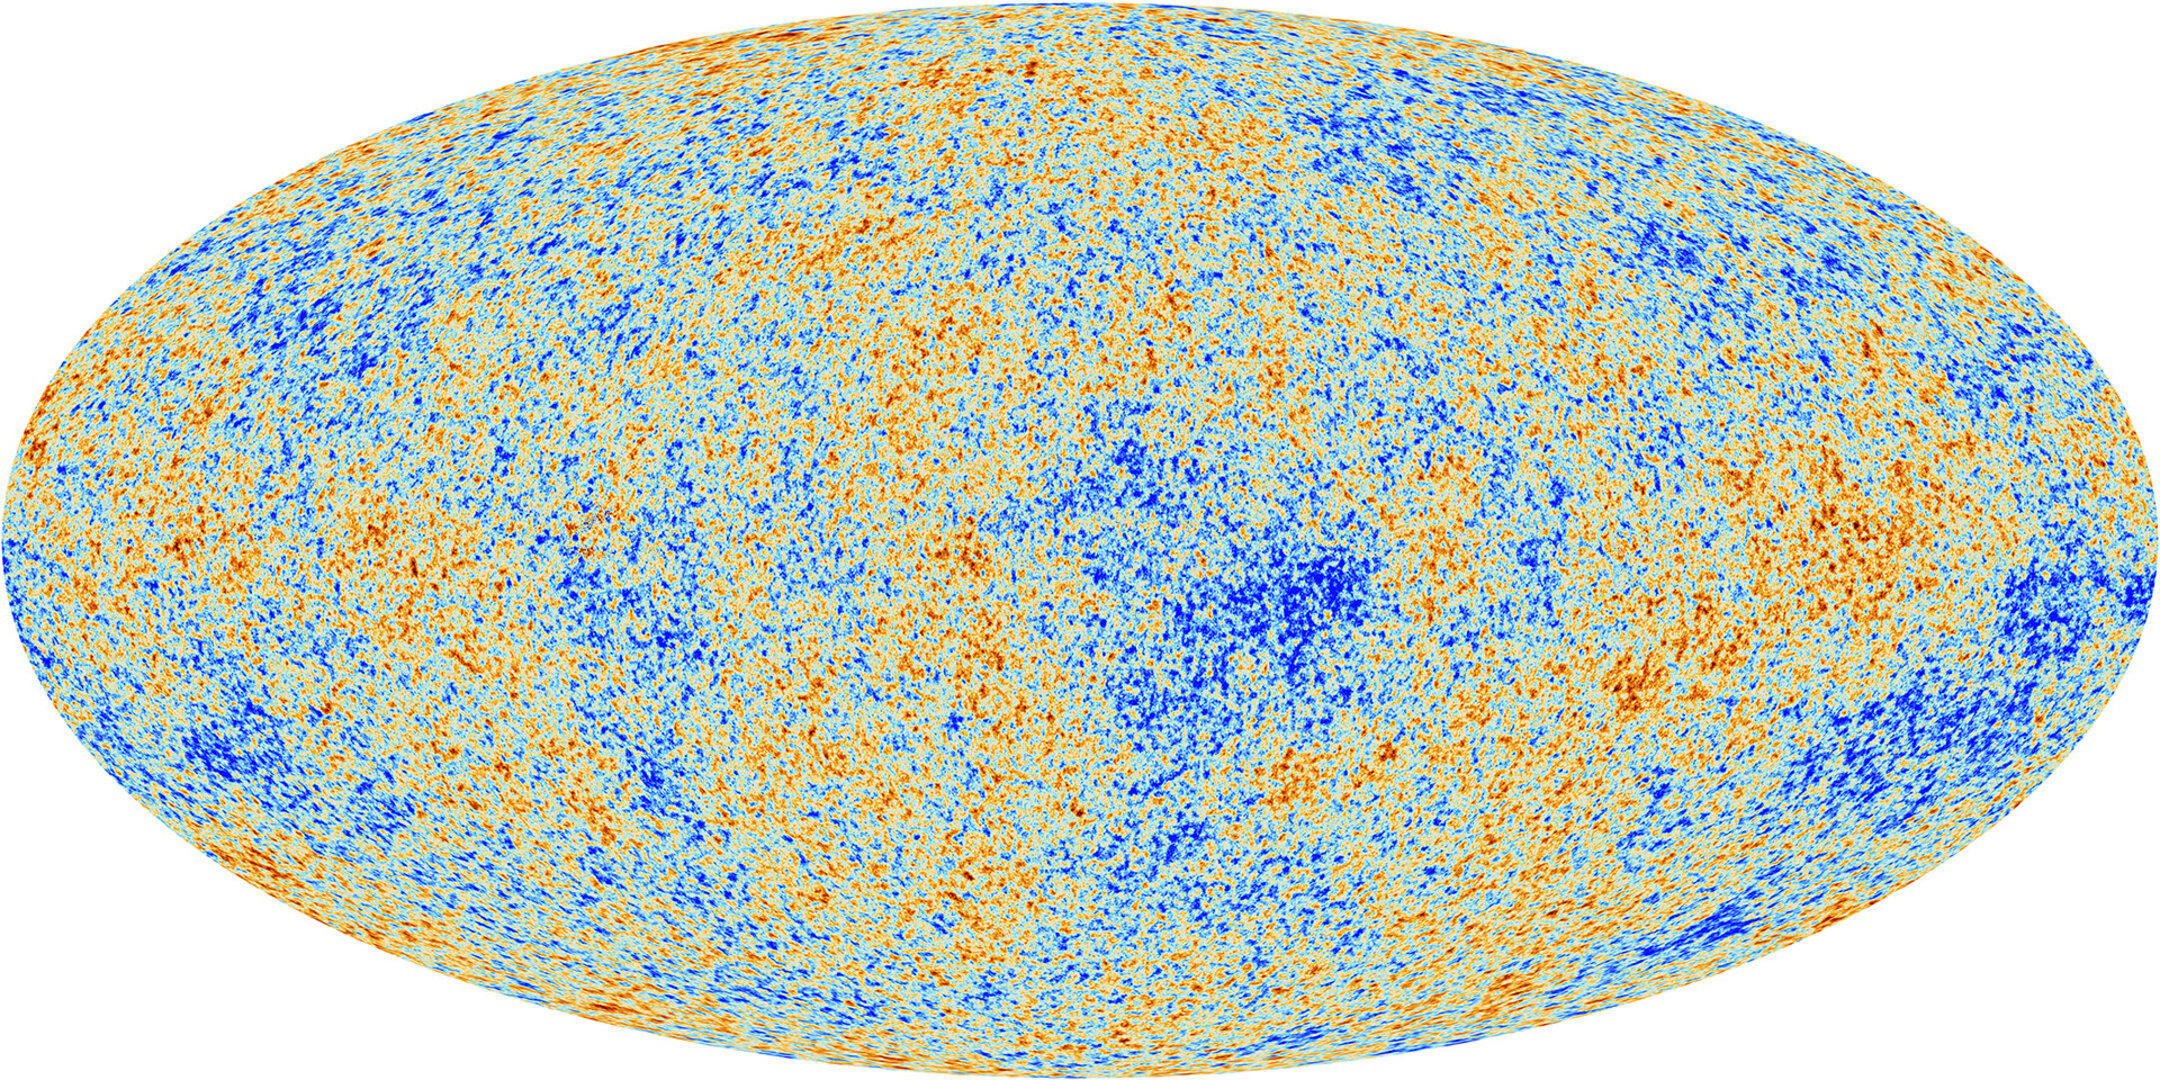
\includegraphics[width=\textwidth]{figures/Planck_satellite_cmb.jpg}

    \end{columns}
\end{frame}

\begin{frame}
    \frametitle{The three pillars of Bayesian inference}
    \begin{itemize}
        \item Parameter estimation: ``What do the data tell me about my model?'':
            \[ \C[0]{P(\theta|D,M)} = \frac{\C[2]{P(D|\theta,M)} \C[1]{P(\theta|M)}}{\C[3]{P(D|M)}}, \qquad \C[0]{\mathcal{P}} = \frac{\C[2]{\mathcal{L}} \times\C[1]{\pi}}{\C[3]{\mathcal{Z}}}, \qquad \C[0]{\text{Posterior}} = \frac{\C[2]{\text{Likelihood}} \times\C[1]{\text{Prior}}}{\C[3]{\text{Evidence}}}. \]
        \item Model comparison: ``Which model best fits the data?'':
            \[ \C[4]{P(M|D)} = \frac{\C[3]{P(D|M)} \C[5]{P(M)}}{\C[6]{P(D)}}, \qquad \frac{\C[3]{\mathcal{Z}_\mathcal{M}} \C[5]{\Pi_\mathcal{M}}}{\C[6]{\sum_m Z_m \Pi_m}}, \qquad \C[4]{\text{Model Posterior}} = \frac{\C[3]{\text{Evidence}} \times\C[5]{\text{Model Prior}}}{\C[6]{\text{Normalisation}}}.\]
        \item Tension quantification: ``Are datasets consistent within a given model?'' \arxiv{1902.04029}
        \[ \mathcal{R} = \frac{\mathcal{Z}_{AB}}{\mathcal{Z}_A\mathcal{Z}_\mathcal{B}}, \qquad \log\mathcal{S} = \av[\mathcal{P}_{AB}]{\log\mathcal{L}_{AB}}-\av[\mathcal{P}_{A}]{\log\mathcal{L}_{B}}-\av[\mathcal{P}_{B}]{\log\mathcal{L}_{B}}  \]
    \end{itemize}
\end{frame}

%\begin{frame}
%    \frametitle{Foregrounds and parametric models}
%    \begin{columns}[t]
%        \column{0.5\textwidth}
%        \begin{block}{CMB}
%            \begin{itemize}
%                \item 
%            \end{itemize}
%        \end{block}
%        \column{0.5\textwidth}
%        \begin{block}{21-cm global}
%            \begin{itemize}
%                \item 
%            \end{itemize}
%        \end{block}
%    \end{columns}
%\end{frame}

\begin{frame}
    \frametitle{What is a model?}
    \begin{itemize}
        \item Model comparison in its purest form answers question such as:
            \begin{itemize}
                \item ``Is the universe $\Lambda$CDM?''
                \item ``Are neutrinos in a normal or inverted hierarchy?''
                \item ``Is there a detectable global signal in this data?''
            \end{itemize}
        \item However model $\mathcal{M}$ is likelihood $\C[2]{\mathcal{L}=P(D|\theta,M)}$ and priors $\C[1]{\pi=P(\theta|M)}$, $\C[5]{\Pi=P(M)}$
        \item Can use the evidence \C[3]{$\mathcal{Z}$} to decide on which out of a set of likelihoods best describe data (e.g. Gaussian, Cauchy, Poisson, radiometric).
        \item Can also use it for antenna selection~\arxiv{2106.10193}~\arxiv{2109.10098}.
        \item In principle can use it to decide between theoretically motivated priors (care needed)
        \item It can also be used for non-parametric reconstruction:
            \begin{itemize}
                \item ``How many polynomial terms best describe the data?''
                \item ``How complicated a sky model do I need?''
                \item ``Which is the best sky model?''
            \end{itemize}
    \end{itemize}
\end{frame}

\begin{frame}
  \frametitle<1-5>{Primordial power spectrum $\PR(k)$ reconstruction~\arxiv{1908.00906}}
  \frametitle<6>{0 internal knots}
  \frametitle<7>{1 internal knot}
  \frametitle<8>{2 internal knots}
  \frametitle<9>{3 internal knots}
  \frametitle<10>{4 internal knots}
  \frametitle<11>{5 internal knots}
  \frametitle<12>{6 internal knots}
  \frametitle<13>{7 internal knots}
  \frametitle<14>{Bayes Factors}
  \frametitle<15>{Marginalised plot}
  \frametitle<16>{Kullback-Liebler divergences}
  %\framesubtitle{Primordial power spectrum $\PR(k)$ reconstruction}



  \begin{columns}
      \column{0.5\textwidth}
      \uncover<1->{
          \begin{itemize}
              \item Traditionally parameterise the primordial power spectrum with $(A_s,n_s)$
                  \[\mathcal{P}_\mathcal{R}(k) = A_s \left( \frac{k}{k_*} \right)^{n_s-1}\]
              \item To add more degrees of freedom, can add ``running'' parameters $n_\mathrm{run}$ (higher order polynomial in index)
              \item Alternative non-parametric technique introduces a more flexible phenomenological parameterisation: ``FlexKnots''
              \item Let the Bayesian evidence decide when you've introduced too many parameters
          \end{itemize}
      }
      \column{0.5\textwidth}

      \only<1-5>{
  \resizebox{\textwidth} {!} {%
    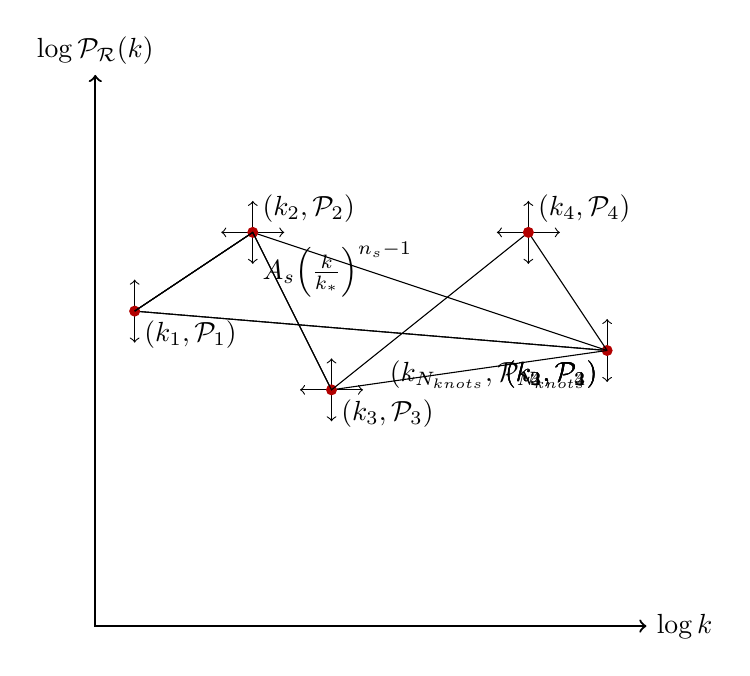
\begin{tikzpicture}
    % width of axes
      \def\xwidth{7}
      \def\ywidth{7}
    % min coordinate
      \def\xmn{0.5}
      \def\ymn{4}
    % start coordinate
      \def\xstart{2}
      \def\ystart{5}
    % middle coordinate
      \def\xmid{3}
      \def\ymid{3}
    % end coordinate
      \def\xend{5.5}
      \def\yend{5}
    % max coordinate
      \def\xmx{6.5}
      \def\ymx{3.5}

    % length of crosses
      \def\croslen{0.4}


    % Draw axes
      \draw<1-5> [<->,thick] (0,\ywidth) node (yaxis) [above] {$\log\PR(k)$}
      |- (\xwidth,0) node (xaxis) [right] {$\log k$};
    % Draw limits
      %\draw [-,dashed] (\xmn,0) node[below] {$\log_{10}k_1$} -- (\xmn,\ywidth) ;
      %\draw [-,dashed] (\xmx,0) node[below] {$\log_{10}k_N$} -- (\xmx,\ywidth) ;

      \draw<1> (\xmn,\ymn) -- (\xmx,\ymx);
      \draw<1> (\xstart,\ystart) node[below right] {$A_s {\left(\frac{k}{k_*}\right)}^{n_s-1}$};

    % Draw the line joining start and end

      \coordinate (mn) at (\xmn,\ymn);
      \coordinate (start) at (\xstart,\ystart);
      \coordinate (mid) at (\xmid,\ymid);
      \coordinate (end) at (\xend,\yend);
      \coordinate (mx) at (\xmx,\ymx);
      \draw<2> (mn) -- (mx);
      \draw<2-5> (mn) node[below right]    {$(k_1,\Pknotj{1})$};
      \draw<2> (mx) node[below left]     {$(k_{2},\Pknotj{{2}})$};
      \onslide<2-5>{\movablevert{mn}};
      \onslide<2-5>{\movablevert{mx}};

      \draw<3> (mn) -- (start) -- (mx);
      \onslide<3-5>{\movablecross{start}};
      \draw<3-5> (start) node[above right] {$(k_2,\Pknotj{2})$};
      \draw<3> (mx) node[below left]     {$(k_{3},\Pknotj{{3}})$};
 
      \draw<4> (mn) -- (start) -- (mid) -- (mx);
      \onslide<4-5>{\movablecross{mid}};
      \draw<4-5> (mid) node[below right] {$(k_3,\Pknotj{3})$};
      \draw<4> (mx) node[below left]     {$(k_{4},\Pknotj{{4}})$};

      \draw<5> (mn) -- (start) -- (mid) -- (end) -- (mx);
      \onslide<5>{\movablecross{end}};
      \draw<5> (end) node[above right] {$(k_4,\Pknotj{4})$};
      \draw<5> (mx) node[below left]     {$(k_{\Nknots},\Pknotj{{\Nknots}})$};


      %\draw<2-> (\xmn,\ymn) coordinate (mn) -- (\xstart,\ystart) coordinate (start) -- (\xmid,\ymid) coordinate (mid) --  (\xend,\yend) coordinate(end) -- (\xmx,\ymx) coordinate(mx);

    % Draw the point labels
      %\draw<2-> (mn) node[below right]    {$(k_1,\Pknotj{1})$};
      %\draw<2-> (start) node[above right] {$(k_2,\Pknotj{2})$};
      %\draw<2-> (mid) node[below right]   {$(k_3,\Pknotj{3})$};
      %\draw<2-> (end) node[above right]   {$(k_4,\Pknotj{4})$};
      %\draw<2-> (mx) node[below left]     {$(k_{\Nknots},\Pknotj{{\Nknots}})$};

    % Draw a dashed line indicating the coordinate names
      %\draw[dashed] (yaxis |- start) node[left] {$y_{1}$}
      %-| (xaxis -| start) node[below] {$x_1$};
      %\draw[dashed] (yaxis |- mid) node[left] {$y_{2}$}
      %-| (xaxis -| mid) node[below] {$x_2$};
      %\draw[dashed] (yaxis |- end) node[left] {$y_{N}$}
      %-| (xaxis -| end) node[below] {$x_N$};
      %\draw  (xaxis -| start) node[below] {$\log_{10}k_2$};
      %\draw  (xaxis -| mid) node[below] {$\log_{10}k_3$};
      %\draw  (xaxis -| end) node[below] {$\log_{10}k_4$};

      % Draw the crosses
      %\onslide<2->{\movablevert{mn}
      %\movablecross{start}
      %\movablecross{mid}
      %\movablecross{end}
      %\movablevert{mx}
    %};

    % put some ellipses in between the start and end point

    \end{tikzpicture}

  }
  }




    \includegraphics<6>[width=\textwidth]{figures/pps_both_1}
    \includegraphics<7>[width=\textwidth]{figures/pps_both_2}
    \includegraphics<8>[width=\textwidth]{figures/pps_both_3}
    \includegraphics<9>[width=\textwidth]{figures/pps_both_4}
    \includegraphics<10>[width=\textwidth]{figures/pps_both_5}
    \includegraphics<11>[width=\textwidth]{figures/pps_both_6}
    \includegraphics<12>[width=\textwidth]{figures/pps_both_7}
    \includegraphics<13>[width=\textwidth]{figures/pps_both_8}
    \includegraphics<14>[width=\textwidth]{figures/pps_evidence}
    \includegraphics<15>[width=\textwidth]{figures/pps_both}
    \includegraphics<16>[width=\textwidth]{figures/DKL.pdf}

  \end{columns}
\end{frame}

\begin{frame}
    \frametitle{Occam's Razor~\arxiv{2102.11511}}
    \begin{itemize}
        \item Bayesian inference quantifies Occam's Razor:
            \begin{itemize}
                \item \textit{``Entities are not to be multiplied without necessity''} \hfill --- William of Occam
                \item \textit{``Everything should be kept as simple as possible, but not simpler''} \hfill --- ``Albert Einstein''
            \end{itemize}
        %\item Consider the Evidence $\C[3]{\mathcal{Z}\equiv P(D|M)}$: 
        %    \begin{description}[Parameter estimation]
        %        \item [Parameter estimation] normalisation constant
        %        \item [Model comparison] critical update factor for \C[5]{model prior} to \C[4]{model posterior}
        %    \end{description}
        \item Properties of the evidence: rearrange Bayes' theorem for parameter estimation
            \[\C[0]{\mathcal{P}(\theta)} = \frac{\C[2]{\mathcal{L}(\theta)} \C[1]{\pi(\theta)}}{\C[3]{\mathcal{Z}}} \qquad\Rightarrow\qquad \C[3]{\log \mathcal{Z}} = \C[2]{\log\mathcal{L}(\theta)} - \log \frac{\C[0]{\mathcal{P}(\theta)}}{\C[1]{\pi(\theta)}} \]  
        \item Evidence is composed of a ``goodness of fit'' term  and ``Occam Penalty''
    \end{itemize}
    \begin{columns}[t]
        \column{0.5\textwidth}
    \begin{itemize}
        \item RHS true for all $\theta$. Take max likelihood value $\theta_*$:
            \[
                \log \mathcal{Z} = -\chi_\mathrm{min}^2 - \text{Mackay penalty}
            \]
    \end{itemize}
        \column{0.5\textwidth}
    \begin{itemize}
        \item Be more Bayesian and take posterior average to get the ``Occam's razor equation''
            \[
                \boxed{
                    \log \mathcal{Z} = \av[\mathcal{P}]{\log\mathcal{L}} - \mathcal{D}_\mathrm{KL}
            }
            \]
    \end{itemize}
    \end{columns}
    \vfill
    \begin{itemize}
        \item Natural regularisation which penalises models with too many parameters.
    \end{itemize}
\end{frame}

\begin{frame}
    \frametitle{Kullback Liebler divergence}
    \begin{columns}
        \column{0.5\textwidth}
        \begin{itemize}
            \item The KL divergence between \C[1]{prior $\pi$} and \C[0]{posterior $\mathcal{P}$} is is defined as:
                \[\mathcal{D}_\mathrm{KL} = \av[\mathcal{P}]{\log\frac{\mathcal{P}}{\pi}} = \int \mathcal{P}(\theta) \log \frac{\mathcal{P}(\theta)}{\pi(\theta)}d\theta.\]
            \item Whilst not a distance, $\mathcal{D}=0$ when $\mathcal{P}=\pi$.
            \item Occurs in the context of machine learning as an objective function for training functions.
            \item In Bayesian inference it can be understood as a log-ratio of ``volumes'':
                \[ \mathcal{D}_\mathrm{KL} \approx \log \frac{V_\pi}{V_\mathrm{P}}.\]
                (this is exact for top-hat distributions).
        \end{itemize}
        \column{0.5\textwidth}
        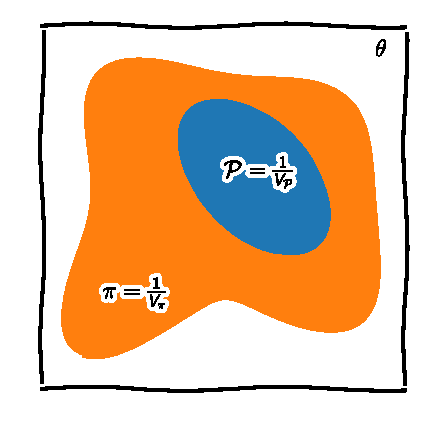
\includegraphics{figures/volumes.pdf}
    \end{columns}
\end{frame}

\begin{frame}
    \frametitle{Why do sampling?}
    \begin{columns}
        \column{0.5\textwidth}
        \begin{itemize}
            \item The cornerstone of numerical Bayesian inference is working with \C[3]{samples}.
            \item Generate a set of representative parameters drawn in proportion to the posterior $\theta\sim\mathcal{P}$.
            \item The magic of marginalisation $\Rightarrow$ perform usual analysis on each sample in turn.
            \item The golden rule is \C[1]{stay in samples} until the last moment before computing summary statistics/triangle plots because \[\boxed{f(\:\av{X}\:)\ne \av{\:f(X)\:}}\]
            \item Generally need $\sim\mathcal{O}(12)$ independent samples to compute a value and error bar.
        \end{itemize}
        \column{0.5\textwidth}
        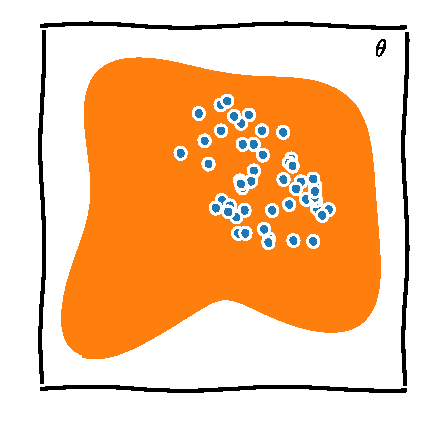
\includegraphics{figures/samples.pdf}
    \end{columns}
\end{frame}

\begin{frame}
    \frametitle{How to generate samples}
    \begin{itemize}
        \item MCMC!
        \item \href{https://chi-feng.github.io/mcmc-demo/}{chi-feng.github.io/mcmc-demo/}
    \end{itemize}
\end{frame}

\begin{frame}
    \frametitle{Nested Sampling: Benefits and drawbacks}
    Relative to traditional numerical posterior samples (Metropolis Hastings, HMC, emcee), nested sampling:
    \begin{description}
        \item[$+$] Can calculate evidence (and therefore perform model comparison).
        \item[$+$] Can calculate KL divergence.
        \item[$+$] Can handle multi-modal distributions.
        \item[$+$] Requires little tuning for an a-priori unseen problem.
        \item[$+$] Highly parallelisable ($n_\mathrm{cores} \sim n_\mathrm{live} \gg 4$).
        \item[$+$] Does not require gradients
        \item[$-$] Slower than a well-tuned posterior sampler.
        \item[$-$] Run time is dependent on prior choice, and priors must be proper \\(some people view this as a feature rather than a bug).
    \end{description}
\end{frame}

\begin{frame}
    \frametitle{Tension quantification}
\end{frame}

\begin{frame}
    \frametitle{Future extensions for REACH}
    \begin{itemize}
        \item Tension quantification for cross validation
        \item Model marginalisation rather than comparison
        \item FlexKnot reconstructions
        \item Likelihood selection
        \item Occam factors on evidence plots.
        \item Integration of calibration and cosmology pipelines
    \end{itemize}
\end{frame}


%\begin{frame}
%    \frametitle{Nested sampling}
%    \cols[0.6]{
%  \begin{itemize}
%    \item Nested sampling is a completely different way of sampling. 
%    \item Uses ensemble sampling to compress prior to posterior.
%      \item Maintain a set $S$ of $n$ samples, which are sequentially updated:
%  \begin{description}
%      
%    \item[$S_0$:] Generate $n$ samples uniformly over the space (from the prior $\pi$). 
%      
%    \item[$S_{n+1}$:] Delete the lowest likelihood sample in $S_{n}$, and replace it with a new uniform sample with higher likelihood
%  \end{description}
% \item Requires one to be able to sample uniformly within a region, subject to a {\em hard likelihood constraint}.
%  \end{itemize}
%    }{
%        \includegraphics<1|handout:0>[width=\textwidth,page=1]{figures/himmelblau}
%        \includegraphics<2|handout:0>[width=\textwidth,page=2]{figures/himmelblau}
%        \includegraphics<3|handout:0>[width=\textwidth,page=3]{figures/himmelblau}
%        \includegraphics<4          >[width=\textwidth,page=4]{figures/himmelblau}
%        \includegraphics<5|handout:0>[width=\textwidth,page=5]{figures/himmelblau}
%        \includegraphics<6|handout:0>[width=\textwidth,page=6]{figures/himmelblau}
%        \includegraphics<7|handout:0>[width=\textwidth,page=7]{figures/himmelblau}
%        \includegraphics<8|handout:0>[width=\textwidth,page=8]{figures/himmelblau}
%        \includegraphics<9|handout:0>[width=\textwidth,page=14]{figures/himmelblau}
%    }
%\end{frame}
%
%
%\begin{frame}
%    \frametitle{Nested sampling}
%    \cols[0.6]{
%  \begin{itemize}
%      \item At the end, one is left with a set of discarded points
%      \item These may be weighted to form posterior samples
%      \item They can also be used to calculate the normalising constant
%          \begin{itemize}
%              \item Critically, this is because nested sampling probabilistically estimates the volume of the parameter space
%                  \[X_i \approx {\left(\frac{n}{n+1}\right)} X_{i-1} \quad\Rightarrow\quad
%                  X_i \approx {\left(\frac{n}{n+1}\right)}^i \approx e^{-i/n} \]
%              \item only statistical estimates, but we know the error bar
%              \item Nested sampling thus estimates the density of states
%              \item it is therefore a partition function calculator
%          \end{itemize}
%      \item The evolving ensemble of live points allows algorithms to perform self-tuning and mode clustering
%  \end{itemize}
%
%    }{
%        \includegraphics<1|handout:0>[width=\textwidth,page=14]{figures/himmelblau}
%        \includegraphics<2          >[width=\textwidth,page=15]{figures/himmelblau}
%    }
%
%\end{frame}
%
%\begin{frame}
%    \frametitle{Implementations of Nested Sampling}
%    %\begin{columns}
%    %    \begin{column}{0.33}
%    %        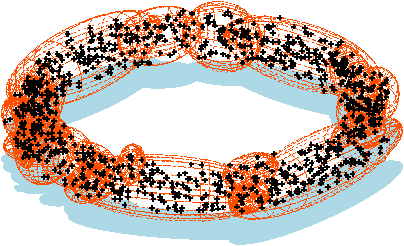
\includegraphics[width=\textwidth]{figures/multinest}
%    %    \end{column} 
%    %\end{columns}
%    \cols[0.5]{%
%        \texttt{MultiNest}
%        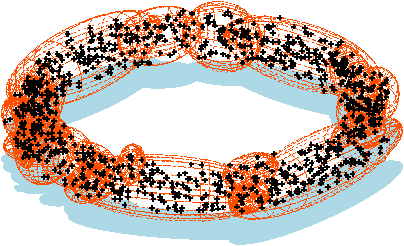
\includegraphics[width=0.8\textwidth]{figures/multinest}
%            \vfill
%        \texttt{DNest}
%        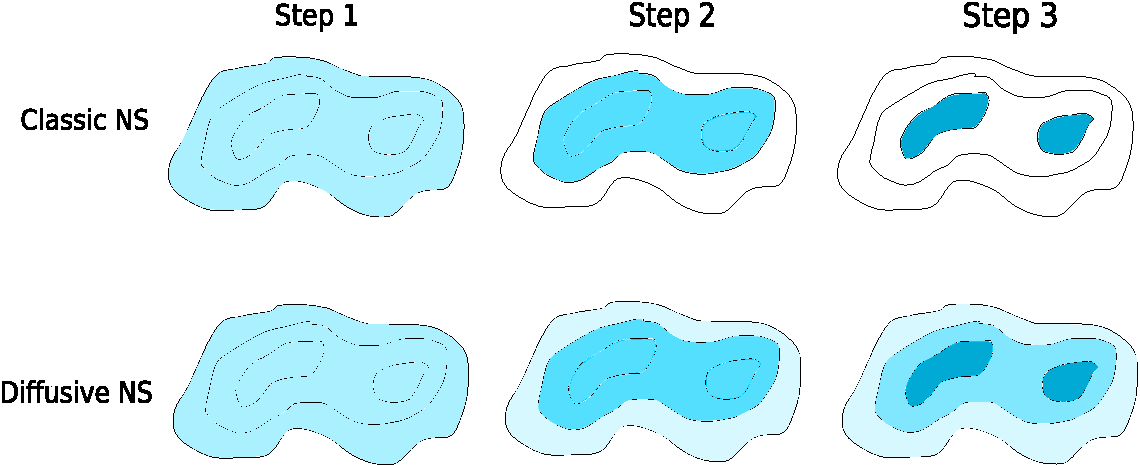
\includegraphics[width=\textwidth]{figures/dnest}
%    }{%
%        \texttt{PolyChord}
%        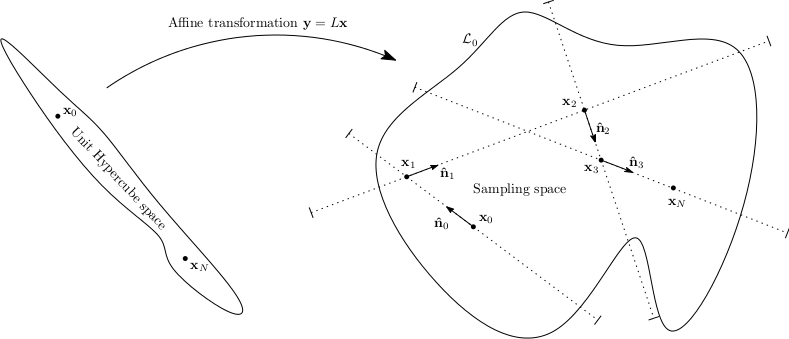
\includegraphics[width=\textwidth]{figures/polychord}
%        \vfill
%        \texttt{NeuralNest}
%            \cols[0.5]{
%                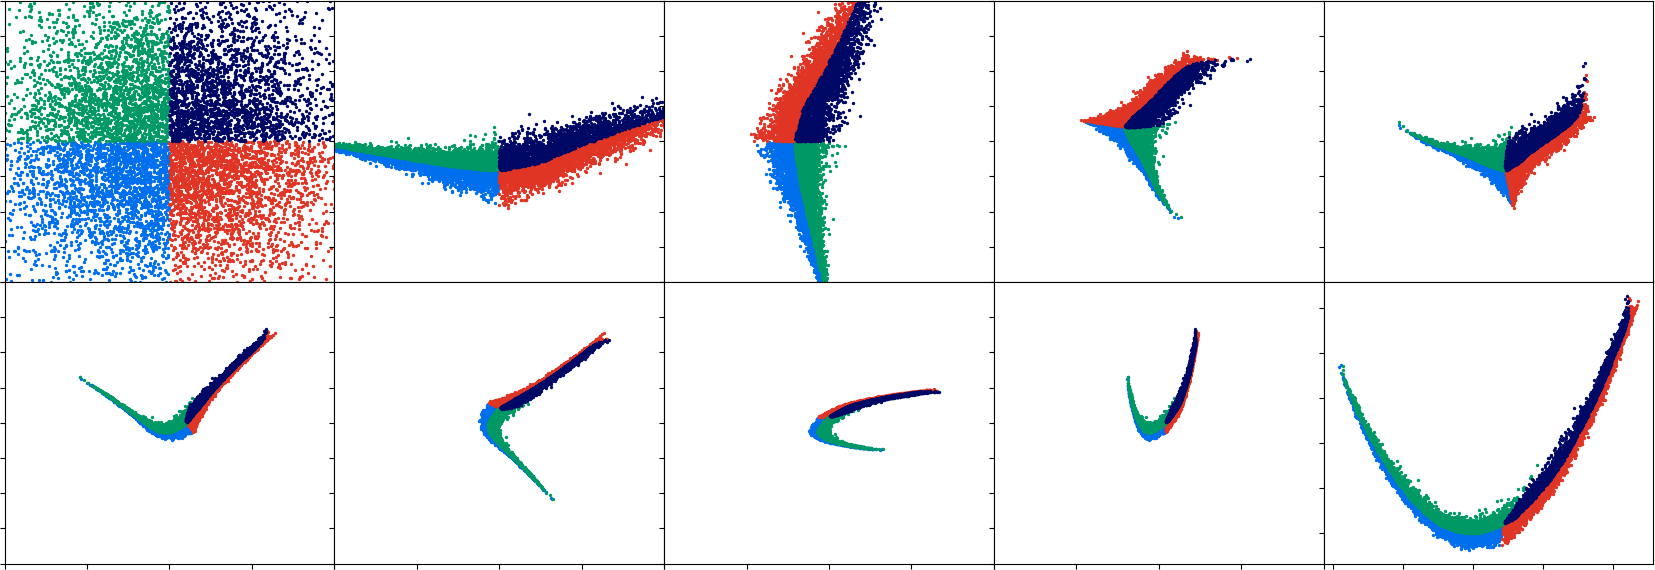
\includegraphics[width=\textwidth]{figures/rosenbrock_flow.png}
%                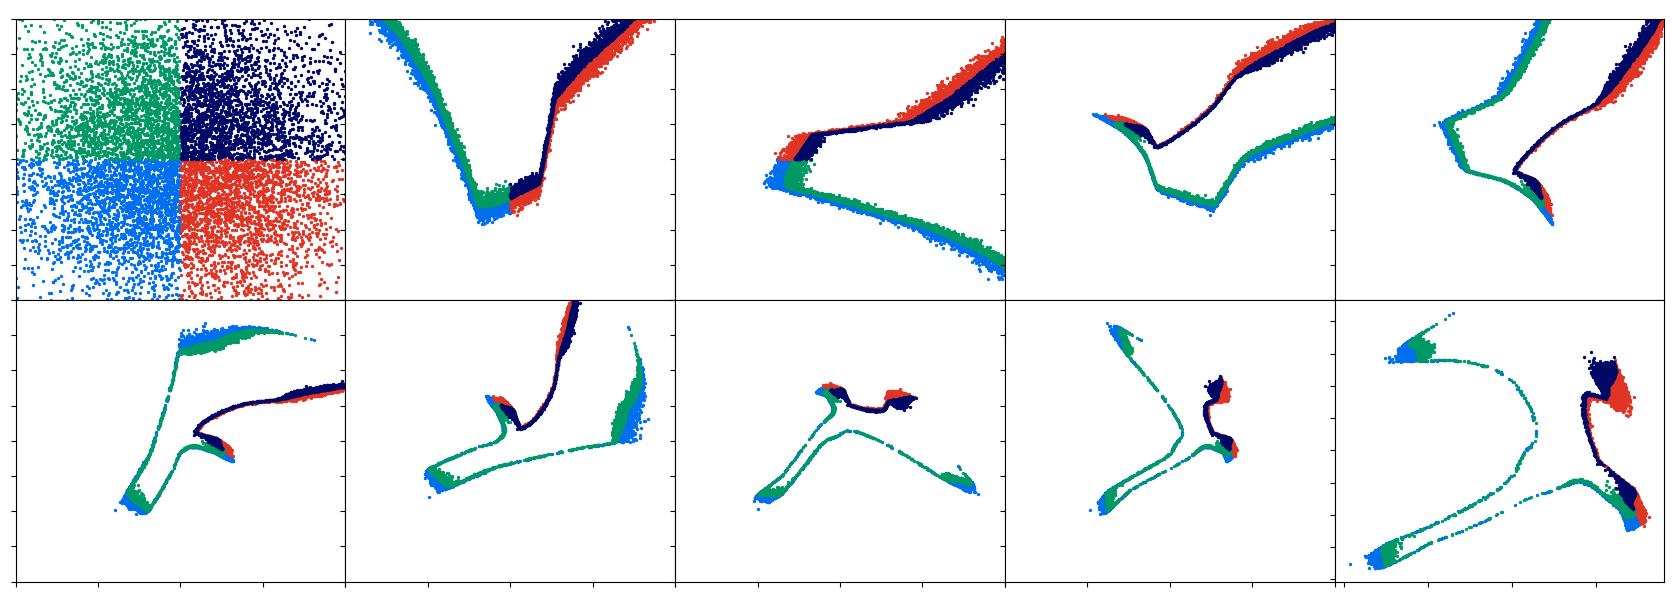
\includegraphics[width=\textwidth]{figures/himmelblau_flow.png}
%            }{
%                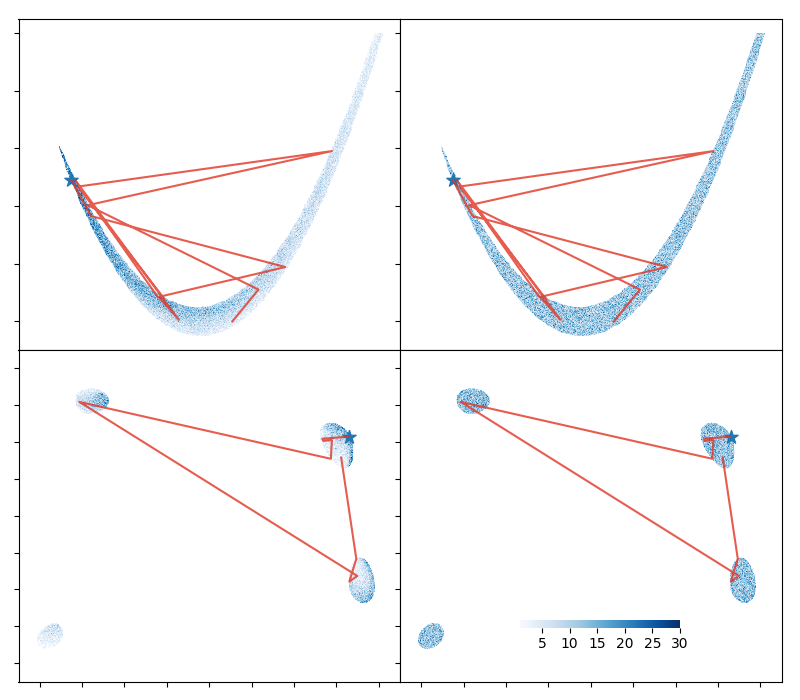
\includegraphics[width=\textwidth]{figures/chains.png}
%            }
%            \vfill
%    }
%\end{frame}
%
%\begin{frame}
%    \frametitle{Nested Sampling: a user's guide}
%    \begin{enumerate}
%        \item Nested sampling is a likelihood scanner, rather than posterior explorer.
%            \begin{itemize}
%                \item This means typically most of its time is spent on burn-in rather than posterior sampling
%                \item Changing the stopping criterion from $10^{-3}$ to $0.5$ does little to speed up the run, but can make results very unreliable
%            \end{itemize}
%        \item The number of live points $n_\mathrm{live}$ is a resolution parameter.
%            \begin{itemize}
%                \item Run time is linear in $n_\mathrm{live}$, posterior and evidence accuracy goes as $\frac{1}{\sqrt{n_\mathrm{live}}}$.
%                \item Set low for exploratory runs $\sim\mathcal{O}(10)$ and increased to $\sim\mathcal{O}(1000)$ for production standard.
%            \end{itemize}
%        \item Most algorithms come with additional reliability parameter(s).
%            \begin{itemize}
%                \item e.g. \texttt{MultiNest}: $\text{eff}$, \texttt{PolyChord}: $n_\mathrm{repeats}$
%                \item These are parameters which have no gain if set too conservatively, but increase the reliability
%                \item Check that results do not degrade if you reduce them from defaults, otherwise increase.
%            \end{itemize}
%    \end{enumerate}
%\end{frame}
%
%
%\begin{frame}
%    \frametitle{Key tools for Nested Sampling}
%    \begin{description}
%        \item[\texttt{anesthetic}] Nested sampling post processing \arxiv{1905.04768}\\
%        \item[\texttt{insertion}] cross-checks using order statistics \arxiv{2006.03371}
%            \hspace{5pt}\url{github.com/williamjameshandley/anesthetic}
%        \item[\texttt{nestcheck}] cross-checks using unthreaded runs \arxiv{1804.06406}\\
%            \hspace{5pt}\url{github.com/ejhigson/nestcheck}
%        \item[\texttt{MultiNest}] Ellipsoidal rejection sampling \arxiv{0809.3437}\\
%            \hspace{5pt}\url{github.com/farhanferoz/MultiNest}
%        \item[\texttt{PolyChord}] Python/C++/Fortran state of the art \arxiv{1506.00171}\\
%            \hspace{5pt}\url{github.com/PolyChord/PolyChordLite} 
%        \item[\texttt{dynesty}] Python re-implementation of several codes \arxiv{1904.02180}\\
%            \hspace{5pt}\url{github.com/joshspeagle/dynesty}
%    \end{description}
%\end{frame}


%\begin{frame}
%    \frametitle{Likelihood free inference}
%    <+Content+>
%\end{frame}

\begin{frame}
    \frametitle{FAQs}
    
    \begin{itemize}
    \item What was that awesome website? \\
    \hfill Full credit to Chi-feng for this incredible online demonstration tool\\
    \hfill \href{https://chi-feng.github.io/mcmc-demo/}{chi-feng.github.io/mcmc-demo/}

    \item How do you make your plots look hand-drawn? \\
        \vspace{5pt}
        \hfill\parbox{0.5\textwidth}{
            \texttt{import matplotlib.pyplot as plt}
            \texttt{ plt.xkcd()}
        }
    \end{itemize}
\end{frame}



\end{document}
